% This is sigproc-sp.tex -FILE FOR V2.6SP OF ACM_PROC_ARTICLE-SP.CLS
% OCTOBER 2002
%
% It is an example file showing how to use the 'acm_proc_article-sp.cls' V2.6SP
% LaTeX2e document class file for Conference Proceedings submissions.
% ----------------------------------------------------------------------------------------------------------------
% This .tex file (and associated .cls V2.6SP) *DOES NOT* produce:
%       1) The Permission Statement
%       2) The Conference (location) Info information
%       3) The Copyright Line with ACM data
%       4) Page numbering
%
%  However, both the CopyrightYear (default to 2002) and the ACM Copyright Data
% (default to X-XXXXX-XX-X/XX/XX) can still be over-ridden by whatever the author
% inserts into the source .tex file.
% e.g.
% \CopyrightYear{2003} will cause 2003 to appear in the copyright line.
% \crdata{0-12345-67-8/90/12} will cause 0-12345-67-8/90/12 to appear in the copyright line.
%
% ---------------------------------------------------------------------------------------------------------------
% It is an example which *does* use the .bib file (from which the .bbl file
% is produced).
% REMEMBER HOWEVER: After having produced the .bbl file,
% and prior to final submission,
% you need to 'insert'  your .bbl file into your source .tex file so as to provide
% ONE 'self-contained' source file.
%
% Questions regarding SIGS should be sent to
% Adrienne Griscti ---> griscti@acm.org
%
% Questions/suggestions regarding the guidelines, .tex and .cls files, etc. to
% Gerald Murray ---> murray@acm.org 
%
% For tracking purposes - this is V2.6SP - OCTOBER 2002


\documentclass[12pt]{article}

\setlength{\oddsidemargin}{0in}
\setlength{\evensidemargin}{0in}
\setlength{\topmargin}{0in}
\setlength{\headheight}{0in}
\setlength{\headsep}{0in}
\setlength{\textwidth}{6in}
\setlength{\textheight}{9in}
\setlength{\parindent}{0in} 

\usepackage{graphicx} %For jpg figure inclusion
\usepackage{times} %For typeface
\usepackage{epsfig}
\usepackage{color} %For Comments
%\usepackage[all]{xy}
\usepackage{float}
%\usepackage{subfigure} 
\usepackage{url}
\usepackage{parskip}

%% Elena's favorite green (thanks, Fernando!)
\definecolor{ForestGreen}{RGB}{34,139,34}
% Uncomment this if you want to show work-in-progress comments
\newcommand{\comment}[1]{{\bf \tt  {#1}}}
% Uncomment this if you don't want to show comments
%\newcommand{\comment}[1]{}
\newcommand{\emcomment}[1]{\textcolor{ForestGreen}{\comment{Elena: {#1}}}}
\newcommand{\todo}[1]{\textcolor{blue}{\comment{To Do: {#1}}}}

\newcommand{\pscomment}[1]{\textcolor{red}{\comment{Paul: {#1}}}}
\newcommand{\mmcomment}[1]{\textcolor{magenta}{\comment{Max: {#1}}}}
\begin{document}
\pagestyle{plain}
%
% --- Author Metadata here ---
%\conferenceinfo{WOODSTOCK}{'97 El Paso, Texas USA}
%\setpagenumber{50}
%\CopyrightYear{2002} % Allows default copyright year (2002) to be
%over-ridden - IF NEED BE. 
%\crdata{0-12345-67-8/90/01}  % Allows default copyright data
%(X-XXXXX-XX-X/XX/XX) to be over-ridden. 
% --- End of Author Metadata ---

\title{Developing a Graphical Library for a Clojure-based Introductory CS Course}
%\subtitle{[Extended Abstract \comment{DO WE NEED THIS?}]
%\titlenote{}}
%
% You need the command \numberofauthors to handle the "boxing"
% and alignment of the authors under the title, and to add
% a section for authors number 4 through n.
%
% Up to the first three authors are aligned under the title;
% use the \alignauthor commands below to handle those names
% and affiliations. Add names, affiliations, addresses for
% additional authors as the argument to \additionalauthors;
% these will be set for you without further effort on your
% part as the last section in the body of your article BEFORE
% References or any Appendices.

\author{
Paul Schliep, Max Magnuson, and Elena Machkasova \\
Computer Science Discipline \\
University of Minnesota Morris\\
Morris, MN 56267\\
schli202@umn.edu, magnu401@umn.edu, elenam@umn.edu
}

\date{}

\maketitle
\thispagestyle{empty}

\section*{\centering Abstract}
This project is a part of an on going effort on adopting the programming language, Clojure, for an introductory college-level CS course.  Clojure is similar to the programming language Racket currently used in an introductory class at UMM, but provides better parallel processing and integration with other programming languages that would benefit students in their future careers. The objective of this project is to develop a beginner-friendly graphical library that focuses on functional approaches to developing programs. We have developed elements of a graphical library that provides the desired functionality, while maintaining a focus on engaging students and key concepts of an introductory CS course, such as problem solving and modularity.  We hope that the developed graphical package, once completed, will be used for an introductory CS course. 


\newpage
\setcounter{page}{1}

\section{Introduction}\label{sec:intro}
%\todo{Overview of project and goals, Paul's section}
UMM offers an introductory CS course on teaching the concepts of problem solving and programming using the language Racket, which is a functional language part of the Lisp family of programming languages designed for students new to programming ~\cite{htdp}. The course utilizes functional approaches of Racket in order for students to better learn the general paradigms of programming. These functional approaches work well to teach students new to programming since functional approaches encourage programming without side effects and emphasize core CS concepts such as recursion. However, since Racket is not often used in real world settings, it does not benefit students as much in their future CS careers. Clojure, which is a functional language also in the Lisp category, offers better concurrency, integration with Java, and is gaining popularity in industry, is a promising candidate for an introductory CS course.  We plan to integrate Clojure into this introductory course in place of Racket because of the benefits it offers, but in order to do so, we need to resolve some of its limitations. One such limitation is Clojure's lack of a fully functional graphical library suitable for an introductory CS course. 

Racket has a full graphical API that is useful for students to create a wide array of programs and also remains consistent with the functional design of Racket. Since graphics are a key motivating component in an introductory CS course, it is important that we implement a graphical API with user-friendly functions for introductory CS students. To fill the gap, we are integrating Quil, an open source graphical environment, into the course ~\cite{Quil}. Quil shows promise since it has a large feature set appropriate for introductory students to create a wide array of graphical programs such as creating a drawing of concentric circles, an animation, or a game. However, Quil was built on top of Java Swing library and it has imperative design approaches to creating programs that would take students out of the functional approaches. It is important that functional approaches remain consistent throughout the course, and having a graphical library with an imperative feel would not be ideal for teaching to beginning CS students. So, to keep the consistency of Clojure's functional approaches and continue teaching the key concepts of the introductory course, we will be creating a graphical set of functions built on top of Quil API that has similar functional approaches as Racket's graphical API. In order to do so, we abstract over many of the functions offered by Quil. While there have been many technical difficulties in working with Quil on creating this graphical set of functions, we have been able to successfully abstract over many of Quil's current functions to create a system that is closer to the functional design of Clojure.

\emcomment{We need to remind the reader about what functional and imperative is.}

\section{Overview of Clojure}\label{sec:clojure}
%\todo{Max's section}
Clojure is a functional programming language in the Lisp family of languages. Clojure was developed by Rich Hickey and released in 2007~\cite{Hickey:2008}. Clojure was developed with a strong emphasis on functional programming with its immutable data types and first class functions. Additionally, Clojure provides a rich set of data structures that are immutable, such as lists, vectors, and hashmaps.
%\mmcomment{I'm not quite sure. Currently we have the explanation of functional approaches near the end of the paper which would be the best spot to explain functional vs imperative, but for a lot of the following sections it requires differentiating between functional and imperative.}

Immutable data types are data types that cannot be changed. In Clojure when a change to an item of data is needed, a new data item will be made with that new value. Immutable data types are useful for avoiding side effects in functions. A side effect is when a function directly manipulates memory or noticeably interacts outside of its own scope other than to return a value. So if a function would change a global variable then it would have a side effect. Side effects can make finding the cause of a problem in code more troublesome. If a function interacts with more than itself then the problem can be spread out through the rest of the program making it more difficult to fix. By reducing side effects, the problems will often be localized and easier to fix. 

\emcomment{explain the syntax}

First class functions are functions that can be passed as arguments into other functions, returned from functions, or stored in data structures.
\begin{verbatim}
	(def square-root[x] (* x x))
	
	(map square-root [1 2 3 4])
	-> (1 4 9 16)
\end{verbatim}
Here the function \texttt{square-root} is defined which takes in a number as an argument and squares it. Then \texttt{square-root} is passed in as an argument to map which takes a function and a collection as arguments and applies the function to each item in the collection. Then the resulting collection is returned.   

\section{Goals and Setup for an Introductory Course}\label{sec:racket-clojure}
\emcomment{Section~\ref{subsec:plans} assumes that we have already talked about Clojure-Java integration and usefulness in the work filed. This may or may not belong here, but it has to be somewhere.}

\pscomment{I added some of the clojure-java integration and usefulness in my section for plans on introducing Clojure.  It can still be added here, but wouldn't be necessary anymore.}

\subsection{Overview of Current UMM CS Introductory Course}\label{subsec:course}
\todo{Elena's subsection}
~\cite{htdp}
~\cite{lein} \emcomment{Look into including URLs}

\subsection{Plans for Introducing Clojure}\label{subsec:plans}
%\todo{Paul's section}
The current UMM introductory CS curriculum uses Racket because of its ease of use and functional design make it beneficial for teaching the learning objectives of an introductory CS course.  However, since Racket is primarily a teaching language and is not often used outside of the classroom environment, it is less beneficial for students in their future work. \pscomment{cut down on this, and be gentle with Racket comments} 
Clojure, however, is better suited for students in their future CS careers as it has integration with Java, better parallel processing, and is gaining popularity in the work field. What also makes Clojure well-suited is that it has functional design similar to that of Racket. Functional design in an introductory course is important since it teaches students many fundamentals of programming and problem solving such as recursion, modularity, and the importance of immutability. The benefit of teaching these concepts using functional approaches over imperative approaches is that functional programming is without side effects because of its immutability and stateless design so that students would not need to worry about managing in-place object changes in an introductory course. Functional programming is well-suited for learning problem solving as well since it teaches students apply different approaches to solving problems and can help students engage in other languages more easily.
\pscomment{some of the previous paragraph might be moved into ~\ref{subsec:course}}

Clojure’s integration with Java and usefulness in the work field are just some of the perks that we feel can be beneficial to students in preparing for their future careers in computer science.  Although Clojure provides many important benefits not seen in Racket, it is not yet a language ready for using in an introductory CS course. Many steps must be taken in order to provide alternative approaches with an easier transition to programming for Clojure's high learning curve that prevents it from being usable for beginner-level CS students.

One barrier preventing Clojure from being used in an introductory CS course is its error messages. Often, they tend to be unintuitive and unnecessarily long and can be hard to understand for experienced programmers, much less beginning CS students. Also, there is not an environment that supports easy navigation of the error messages and connecting them to the location of the offending line of code (such as highlighting that line of code). Since problem solving is a core learning objective of the introductory course, it is essential for error messages to be usable for beginning students to enable them to easily troubleshoot issues and focus on key learning concepts. To solve these issues, we catch the error messages and substitute them with more user-friendly messages appropriate for introductory CS students.
\emcomment{add the reference to tfpie paper}

Along with the lack of an appropriate user interface for error messages, there is also an absence of a complete development environment for beginner programmers to easily program in. %The current UMM introductory CS course that uses Racket integrates an IDE called DrRacket that incorporates a user-friendly interface for students to develop programs in, something that is necessary for an introductory CS course. 
Currently, there is a Clojure IDE that is still in development called Light Table.  Since Light Table was designed for programming in Clojure and was created with usability in mind, it shows promise in usability for introductory computer science students. We are currently exploring ways of integrating our error message handling with Light Table before it can be useful for an introductory course.
\pscomment{Reference Light Table}

A graphical environment in an introductory course provides good motivation for students to explore the language and practice their programming skills. Currently, there is no built-in system for graphical functions in Clojure and there is no beginner-friendly graphical library that teaches the learning objectives of functional programming in an introductory CS course. A potential graphical library to use for programming is an open-source project called Quil that provides a lot of functionality that is needed for a graphical library necessary for students to use in an introductory CS course. Below is an example of a drawing done in Quil picturing a sine wave.

\begin{center}
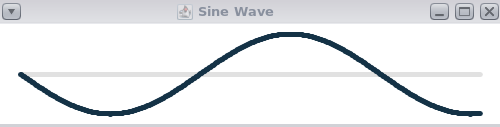
\includegraphics[width=300pt]{sine-wave}
\end{center}

However, there are limitations and potential issues to using this graphical library that would steer away from the learning objectives and functional approaches that UMM's introductory CS curriculum has in place. Our project's goals are to resolve these limitations posed by Quil and have a fully functional graphical library that students may be able to easily use to create interesting and useful programs and still develop their problem solving skills through functional approaches. \pscomment{run on sentence}


\subsection{Requirements for a Graphical Library}\label{subsec:requirements}
\todo{Talk about state and how to handle in a functional way, Max's section}
Racket's graphical library has proven to be a powerful teaching tool in the current UMM CS introductory course by allowing students to make their own animations less than a month into the semester without any prior programming background. This maintains interest in programming while reinforcing key concepts. 

With this in mind, we employed the Quil graphical library.\mmcomment{mention Racket's MVC earlier and transition}

Model-view-controller (MVC) is a way of handling user interfaces. The model updates the collection of data used for displaying graphics. The view is the actual visual representation of the graphics. The view will listen for changes from the model and then reflect that visually. The controller listens for changes and then relays those changes to the model for updating. This modularization of the work greatly reduces the dependency on the order of operations. If everything was updated piece by piece by taking in input, updating the data, then displaying it graphically, then the order of operations of the model, view, and control would all matter simultaneously. Since the process is separated into independent components, the order of operations only matters within each component. Model-view-controller is the system used by Racket's graphical library.

State in Quil is the collection of data related to each graphical object, not the graphical representation itself. Consider a picture of a rocket. The rocket object has certain properties such as position, size, and color. The state of the rocket would be the object that contains this data. The graphical representation of the rocket would use the data stored by state to know where to draw the rocket, how big to draw the rocket, and what color the rocket should be. If the rocket was moving through the air, the state would update the position and possibly the size of rocket. Then, the new rocket would be drawn after the updates are made. In Quil, the process of updating state and drawing the graphics are completed using the same function. Since this process is combined, the order in which steps are taken is very important, and certain processes start caring about other processes that are unrelated. Parts of the state need to be updated before drawing them, and those parts need to be drawn in the correct order in case the layering matters. In this case the order of operations of updating state and drawing the graphics matters at the same time as opposed to the MVC. If we needed to draw a wheel on a car that was moving across the screen, first the tire's properties would be updated then drawn. Then, the rim's properties would be updated and drawn. This order would maintain the shape of the wheel because the tire would not be obscuring the rim. In this example, the order of updating the rim cares about when the tire is drawn. These two processes shouldn't really care about when one or the other is performed. This unnecessarily complicates the process of drawing the wheel and is an inherent flaw in Quil's design from a functional approach. While Quil's system can accomplish needed tasks, it is very imperative in its design which defeats the intent of teaching functional approaches. To address the issues of the imperative design we emulated the model-view-controller system of Racket's graphical library and modularized the process.

\emcomment{This probably should be its own subsection; make the transition clearer: this is the essence of what we are doing; perhaps needs to be later in the paper; need to think about it}
\mmcomment{Yeah, this should probably go in the section Developing a Clojure Graphical Library. It seems like Paul and I both go into a bit of detail of our changes to Quil, and it might be better to have it in its own separate section probably after functional approaches.}
In our design of the graphical library we needed to separate the processes of updating state and displaying state. In order to accomplish this we developed a system that would take in as setup:
\begin{itemize}
	\item A collection of graphics variables
	\item A collection of functions to update state
	\item An ordered collection of functions used to display graphics
\end{itemize}
Example of user code in our graphical library design
\begin{verbatim}
(def states 
	{:snake [450 450 450 470 450 490 450 510] :snakeHeadX 450 
	:snakeHeadY 450 :foodX 150 :foodY 150 :snake-direction "north" 
	:foodExists false :score 0}
)
(def updates
	{:setup-drawing setup :update-snake update-snake}
)
(def display-order
	[draw-snake draw-food redraw-canvas]
)
\end{verbatim}
This code is for a game of snake. \texttt{States} is a hashmap with data that is required for drawing the graphical representation of the game. \texttt{Updates} is a hashmap containing functions that are designed by the user that will be used to update the state. Finally, \texttt{display-order} is a collection of functions designed by the user to draw the different parts of the game in order. The order being the first item in the collection will be the top layer, in this case the snake which will be drawn last, and the last item is the last layer, in this case being the background which will be drawn first.

\begin{center}
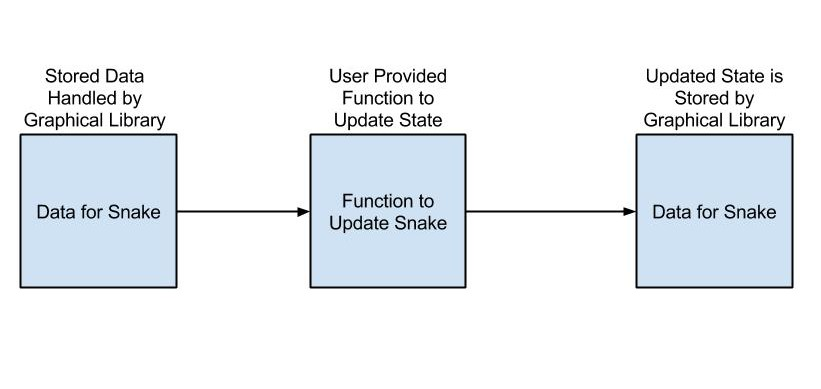
\includegraphics[width=300pt]{Handling_State_in_Graphical_Library}
\end{center}
 
This design accomplishes both abstracting over direct memory manipulation and making order of operations matter less. Our design abstracts over direct memory manipulation by taking care of changing variables for the user. When a part of the state is ready for updating our system will input the stored data as an argument into the update function then take the newly updated state and store that data. The accessing of the data and the storing of the data is all handled by the system and not by the user. When the graphics are displayed the data is accessed again by our system and given to the user made function to draw the graphics. 

Our design makes order of operations matter less by encapsulating updating state and displaying state. In Quil, a single draw function is used to do everything. That draw function is supposed to update state and draw everything. This is a messy process that heavily relies on order of operations, and causes a lot of inter-dependencies that really should not be an issue. Updating is happening intermittently as drawing is happening, so updating of certain data can become dependent on displaying certain graphics that are inherently unrelated. We alleviate this issue by separating update and display into separate processes. All of the updating of state will be done prior to displaying a single graphic. Therefore, only the order in which the graphics are displayed will matter. This order cannot be removed entirely due to the nature of graphics. If a car wheel is being displayed, the tire would need to be drawn before the rim. Otherwise, the rim would be completely obscured by the tire.

\section{Developing a Clojure Graphical Library}\label{sec:library}



\subsection{Overview of Quil}\label{subsec:quil}
\todo{technical difficulties, imperative approaches, etc. Paul's section}
Graphics are an important aspect on teaching students the basis for programming in an introductory CS course. They give students a visual representation of data in their programs and give an appealing incentive to practice their programming skills, problem solving, and develop a sense of functional approaches. To provide a graphical library for students, we utilize an open-source graphical library called Quil.

Quil is an open-source graphical API developed for creating functions that display and transform graphical elements in Clojure. It provides the user a library of functions such as creating shapes or changing colors that can be used for an array of projects for students in an introductory-level CS course. These projects can range from creating a drawing of a sine wave to a game such as tic tac toe. Since Quil is built on top of Java Swing, it uses Java applets to display the graphical images and updates them constantly using a system of a set of frames that the user manipulates in order to animate drawings. However, Quil has some limitations that prevent it from being usable for an introductory CS course that teaches introductory students functional approaches to programming.

An apparent limitation of Quil is it has imperative approaches and functionality that would not be acceptable for students to learn in a class based on functional programming. For example, when manipulating the world state in Quil, the state is first set, then the state is displayed and updated simultaneously in a draw function, which directly manipulates memory from the state and goes against the model-view control of functional programming. In order to keep the consistency of the functional approaches of Clojure, we are working on creating a graphical library of functions with design that implements functional approaches similar to Racket’s graphical library that abstracts over Quil's functionality. There have been many technical difficulties imposed by Quil in attempting to create this graphical library.

Developing programs in Quil's environment involves creating a setup function for setting the initial background color, setting the frame rate, etc; developing a draw function for creating shapes and colors that will be transformed as necessary; and putting these functions into a \texttt{defsketch}, a macro that calls these functions as well as creating the title and size of the window. In order for Quil to be able to run programs, the user must use the \texttt{defsketch} for the work to be displayed.
\begin{verbatim}
(defsketch example    ;; Define a new sketch named example
 :title "Example"    ;; Set the title of the sketch
 :setup setup        ;; Specify the setup fn
 :draw draw          ;; Specify the draw fn
 :size [500 400])    ;; Specify the size of the window
\end{verbatim}
Our first step to create a more functional library was to separate the state manipulation so that it’s called through three separate entities: set, update, and display. However, since Quil requires the user calling \texttt{defsketch} in order to call the functions of the program where the state is also manipulated, it posed issues on trying to create the desired functional system of state. 

Another challenged we faced when developing our functional library is that although Quil does feature some documentation on its functions, installation, and examples, it was still under-documented enough to where it caused issues for our initial use. This also posed issues when making new functions that abstract over the current ones. This includes both the API’s documentation as well as the documentation within the source code. So, when trying to understand how many of the functions worked (such as its system of state), we had to scour the source code and look at how the functions are set up to find a proper answer. 

In order to overcome the challenges of developing our desired functional system state, we plan to hide the \texttt{defsketch} program by making it auto generated by a macro. This is necessary since \texttt{defsketch} takes the user out of the functional programming and would help us create the system of state where memory manipulation would be able to be more easily abstracted over. Also, to ensure students won’t have an issue finding information about the functions, we plan to ensure that our graphical library will have a full API that details each function as well as appropriate examples for each. 

\subsection{Introducing Functional Approaches}\label{subsec:functional}
%\todo{Max's section}
Functional approaches to programming are stylistic choices that utilize the structure of functional programming. In designing our graphical library we focused on reducing the dependency on order of operations and limiting the need for the user to directly manipulate memory. These are two concepts that are common practice in functional programming.

Functional approaches to programming reduce the dependency on order of operations by using immutable data types and by encapsulating functions. If two functions needed to access the same field and change it throughout the functions' evaluation, the order in which these functions operate would heavily depend upon each other since they are using the same field. If one function is accessing the field after the other has changed it, then the value the function receives would be different than the expected value. This is avoided by using immutable data types. The field would be passed around as an immutable data type, and when ever a change to it is needed a new instance would be created. This style is more in line with functional approaches to programming. Another way to reduce dependency on order of operations is by encapsulating functions. If functions reduce the amount of interactions with other functions and are broken down into their specific roles, then order starts to matter less. Consider a wheel moving across a screen. If a single function took the role of moving that wheel across the screen, then that function would need to update the position of each part of the wheel and then draw it. First the position of the tire would need to be updated then drawn. Then the same would need to be down for the rim. In this process the updating of the position of the rim is now dependent on the updating of the position of the tire due to the order of operations. If we split this process up into an update function and a draw function then this dependency would not longer exist. Everything could be updated in the update function in whatever order since nothing has been displayed yet. Then the draw function would draw the tire followed by the rim. Even in this small example, by encapsulating the functions of update and draw, dependency on order of operations is reduced. If this were done for an entire car, the result would have an even greater effect.

The other concept we focused on is reducing the need for the user to directly manipulate memory. Functional approaches achieve this by using immutable data types and making functions free of side effects. A side effect in programming is when a function does something to interact with anything outside of that function with the exception of returning a value. If a function is called that accesses a field, changes it, and then returns a value, then the function would be considered to have a side effect. Immutable data types are perfect for solving this issue. A data type can be passed in to the function, a new version of it can be produced, and then returned. No interacting with global variables or fields. No changing its arguments. Directly manipulating memory is avoided entirely. Therefore, there will be no side effects. 

\section{Examples of Usage of the Graphical Library}\label{sec:usage}
\todo{Add examples as we are writing.  Make it into a section once we know what's in it.}

\section{Conclusions and Future Work}\label{sec:future-work}
We have managed to abstract over many of the functions and imperative approaches from Quil and have started to create a system that reflects the functional design of Clojure. With our system, students can easily create programs using functional approaches to produce graphical figures. This is made possible through our emulation of Racket’s model-view-controller system.  
While our developed graphical library accomplishes many of our design goals, it still has some work left before it can be considered ready for an introductory CS course. We plan to abstract over the \texttt{defsketch} function with our own macro in order to make it work with our developed code for state. We also plan to write documentation for our developed functions and system as well as examples. We will continue to abstract over functions that we deem to be inaccessible to introductory CS students. After the project is ready, we plan to make tests for the system in order to ensure it is ready for the introductory CS course.  


%
% The following two commands are all you need in the
% initial runs of your .tex file to
% produce the bibliography for the citations in your paper.
%\bibliographystyle{abbrv}
%\end{thebibliography}

%\bibliography{generic_types}  
% You must have a proper ".bib" file
%  and remember to run:
% latex bibtex latex latex
% to resolve all references
%
% ACM needs 'a single self-contained file'!
%
\bibliographystyle{ACM}
\bibliography{mics2014introclass}


% That's all folks!
\end{document}

%%%%%%%%%%%%%%%%%%%%%%%%%%%%%%%%%%%%%%%%%%%%%%%%%%%%%%%%%%%%%%%%
